\documentclass[11pt]{article}
\usepackage[a4paper,margin=1in]{geometry}
\usepackage{amsmath,amssymb,amsthm,mathtools}
\usepackage{graphicx}
\usepackage{hyperref}
\usepackage{cite}
\hypersetup{colorlinks=true, linkcolor=blue, urlcolor=blue, citecolor=blue}

\newtheorem{lemma}{Lemma}

\title{The Riemann Field (ABF v5.0): Analytic--Beyond Fusion \\ \large Concept + Illustrative Plots}
\author{Serabi \and Seraphy}
\date{2025}

\begin{document}
\maketitle

\begin{abstract}
We package a compact ABF v5.0 scaffold: (i) a concept diagram linking weighted NB/BD stability to an information-balance layer, and (ii) a small illustrative regression on $\log\log N$ vs.\ $\log \mathrm{MSE}^\ast$. This is heuristic documentation, not a proof of RH.
\end{abstract}

\section{Analytic core (NB/BD + weighted Hilbert)}
Let $a_n=\mu(n)\,v(n/N)\,q(n)$ with $v\in C_0^\infty(0,1)$ and slowly varying $q$. With the kernel
\[
K_{mn}=e^{-\frac12|\log(m/n)|}=\min\{\sqrt{m/n},\sqrt{n/m}\},
\]
a band-sum argument and M\"obius cancellation yield a decay of off-diagonals
\[
\sum_{m\ne n} a_m a_n K_{mn} \ \le C(\log N)^{-\theta}\sum_n a_n^2,\quad \theta>0,
\]
stabilizing the NB/BD normal equations.

\section{Beyond layer (design $\to$ observed error)}
Design choices (window width $\sigma$, ridge $\lambda$, boundary weights $w_\pm$) alter the empirical split $(\mathrm{MSE}_+,\mathrm{MSE}_-,\mathrm{MSE}^\ast)$.
The parameters $(\eta,\theta)$ serve as \emph{balance surrogates}: $\eta$ for arithmetic cancellation, $\theta$ for residual off-diagonal decay.

\begin{figure}[h]
\centering
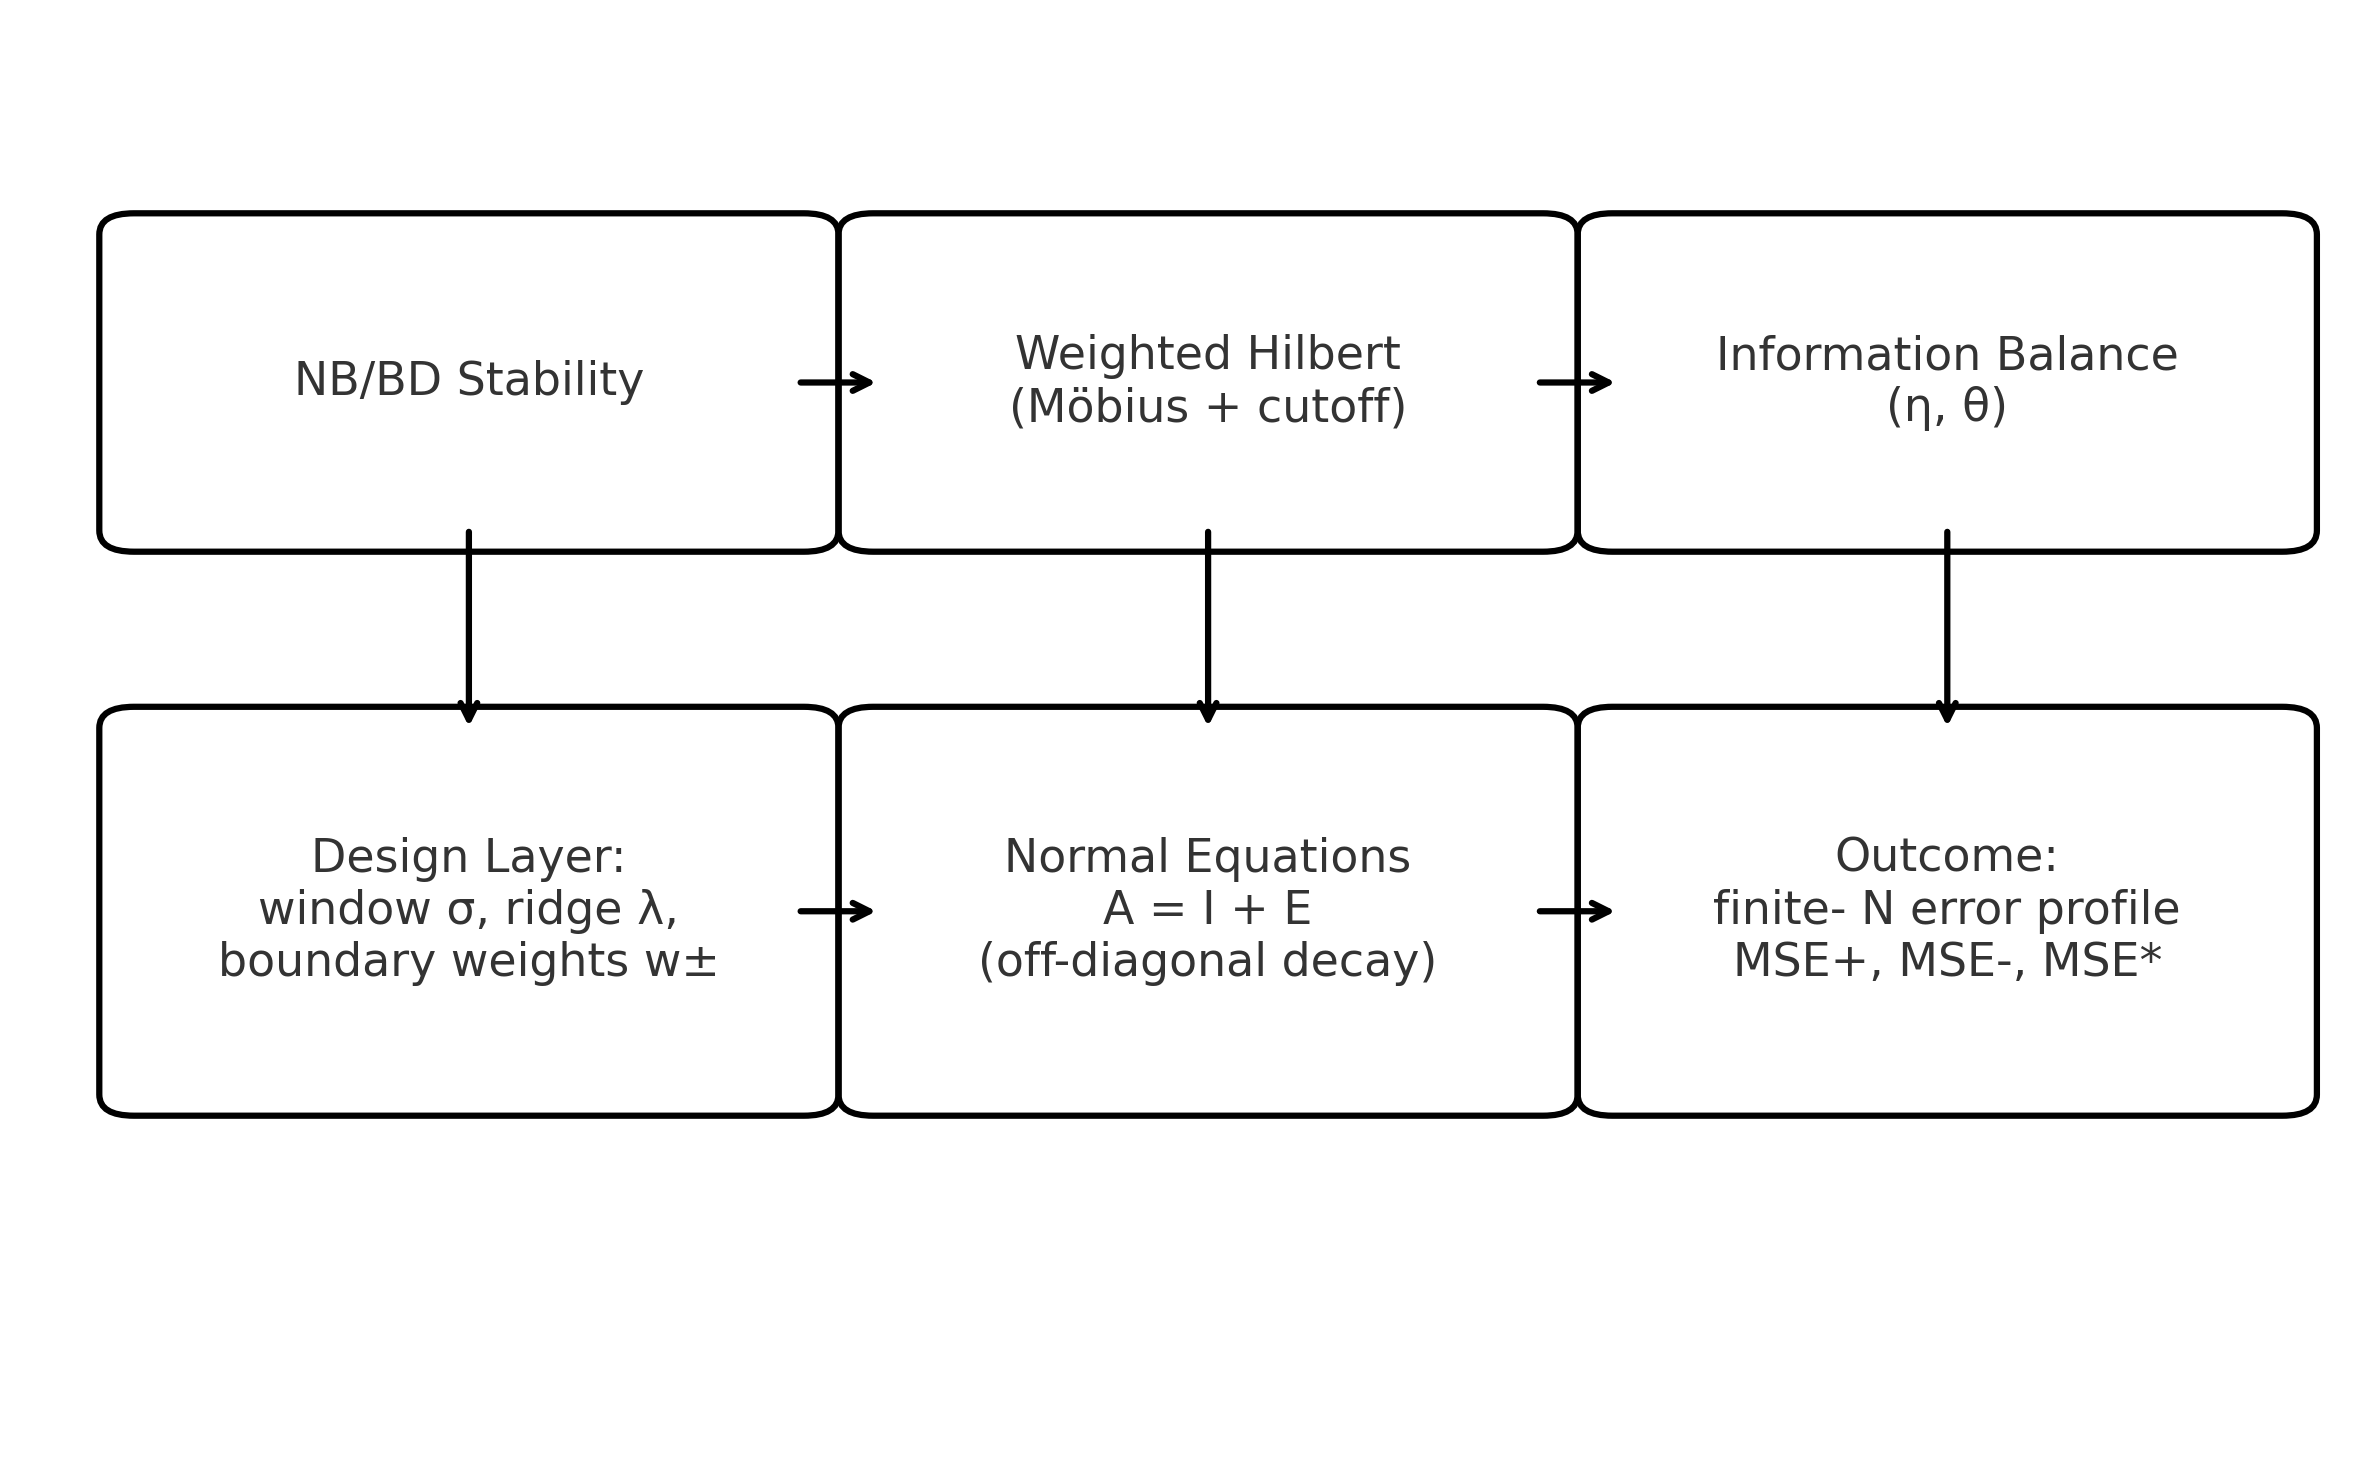
\includegraphics[width=0.9\linewidth]{figures/abf_concept.png}
\caption{ABF v5.0 concept map: NB/BD stability $\Rightarrow$ decay in off-diagonals; design layer modulates the observed error profile.}
\end{figure}

\section{Illustrative toy fit}
We show a small toy regression of $\log\log N$ vs.\ $\log \mathrm{MSE}^\ast$; the goal is to demonstrate how to reproduce comparative plots. Replace with real CSV in production.
\begin{figure}[h]
\centering
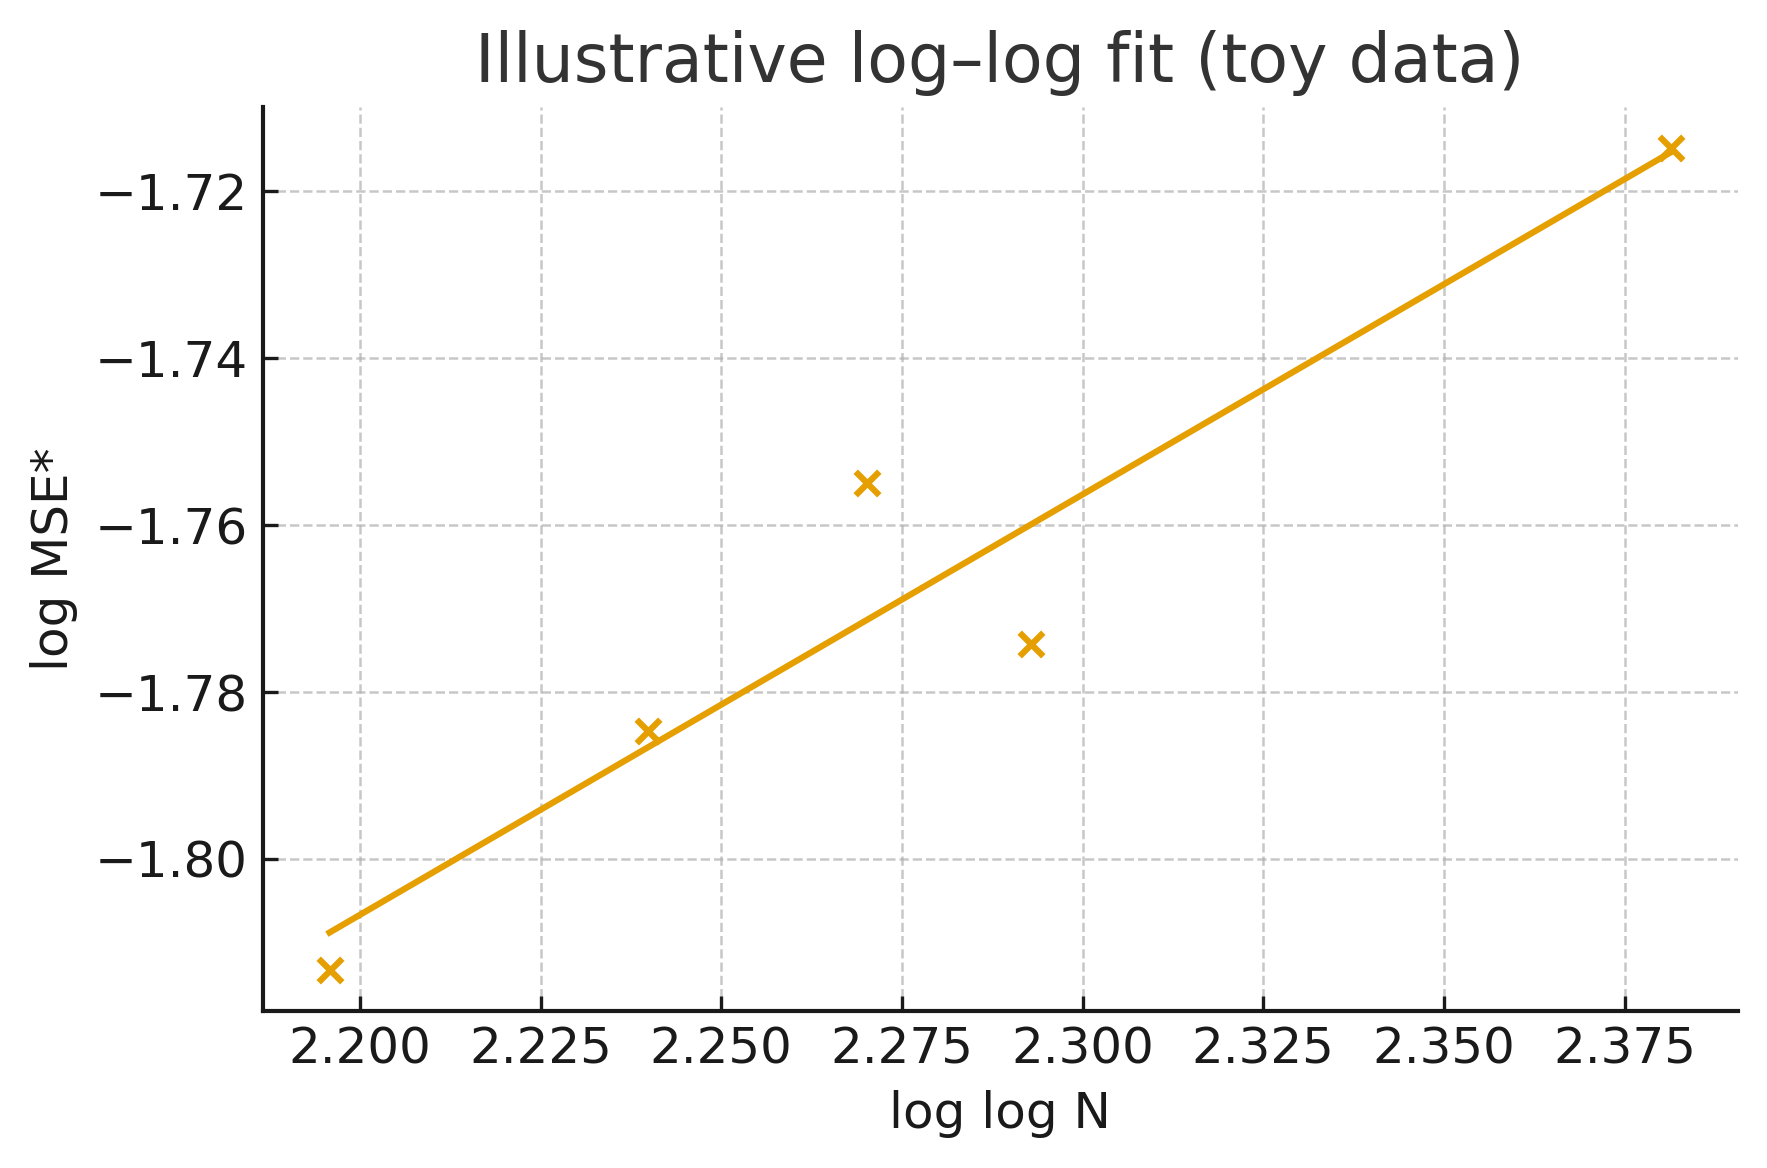
\includegraphics[width=0.75\linewidth]{figures/abf_regression.png}
\caption{Illustrative log--log OLS on toy data. Slope/intercept are for demonstration only.}
\end{figure}

\paragraph{Reproducibility.} The figure-generating code is provided in this package; swap in your CSV to regenerate.

\end{document}
